
\chapter{Implementação Prática de Observabilidade com OpenTelemetry}

\textbf{\textcolor{red}{todo: (texto copiado do documento word), meter cites, italicos e acronimos depois da revisao por parte do orientador}}

\section{Introdução e Caracterização do Sistema Observado}

O cenário atual do desenvolvimento de software é marcado pela crescente adoção de arquiteturas de microsserviços e ambientes cloud-native, com plataformas de gestão como o Kubernetes. Embora essa abordagem promova agilidade, escalabi-lidade e resiliência, ela introduz uma complexidade significativa, especialmente no monitoramento e depuração. A proliferação de serviços distribuídos, cada um com sua própria lógica, e a comunicação assíncrona entre eles, tornam o seguimento de uma única requisição de ponta a ponta uma tarefa desafiadora. Neste contexto, a observabilidade emerge como uma disciplina fundamental para garantir a fiabili-dade, o desempenho e a resiliência desses sistemas (Salah et al., 2017)

\subsection{Visão geral da Arquitetura do Sistema R2UT}

A arquitetura do R2UT segue os princípios das arquiteturas de microserviços para garantir flexibilidade, escalabilidade e resiliência no gerenciamento do ciclo de vida de construção modular. Como apresentado no documento, a plataforma é composta por diversos componentes (ou módulos), cada um responsável por uma funcionalidade específica. A estrutura modular facilita a manutenção, o desenvol-vimento e a implementação de novas funcionalidades sem impactar a operação de outros componentes.
A arquitetura é organizada em camadas, e cada serviço é isolado em um contai-ner Docker, gerido e orquestrado pelo Kubernetes. Isso permite que os serviços sejam executados de maneira autônoma, escalando conforme necessário, e se co-municando por meio de REST APIs, gRPC e mensagens via Kafka. A comunica-ção entre os componentes é feita através de interfaces bem definidas, o que garante um alto nível de desacoplamento entre os microserviços.


% \begin{figure}[H]
% \centering
% \includegraphics[width=0.8\textwidth]{figura3_visaofisica.png}
% \caption{Figura 3 – Visão Física}
% \end{figure}

\subsection{Papel do Kubernetes na Arquitetura do R2UT}

O Kubernetes desempenha um papel central na arquitetura do R2UT, fornecendo a infraestrutura necessária para orquestrar e gerenciar os containers dos microservi-ços, garantindo:

\begin{itemize}
    \item Escalabilidade automática (Auto-scaling): O Kubernetes permite que os pods (unidades de execução de containers) sejam escalados automaticamente com ba-se na carga de trabalho e na demanda de recursos. Isso é essencial para garantir que o sistema possa lidar com picos de uso sem comprometimento de desempe-nho, como no caso de um aumento de utilizadores que acessam simultaneamen-te os serviços;
    \item Alta disponibilidade (High Availability - HA): O Kubernetes garante que, caso um pod falhe, outro seja automaticamente reiniciado em um nó diferente do cluster, minimizando o impacto de falhas no sistema. Isso assegura que os serviços essenciais, como autenticação e autorização, ou até mesmo o gerencia-mento de IoT devices, continuem operando sem interrupção;
    \item Gerenciamento de containers: O Kubernetes gerencia a execução de contai-ners, garantindo que todos os microserviços estejam devidamente implantados e funcionando corretamente. Ele também facilita a atualização e a implementação de novas versões dos serviços, sem tempo de inatividade, por meio do rolling update;
    \item Orquestração e balanceamento de carga: O Kubernetes pode ser configurado para balancear automaticamente a carga de trabalho entre diferentes réplicas de um serviço, garantindo que o tráfego seja distribuído de maneira eficiente, sem sobrecarregar nenhum servidor individualmente. Essa orquestração é crucial pa-ra garantir que as interações entre os microserviços sejam rápidas e confiáveis.
\end{itemize}

\subsection{Arquitetura de Microserviços no Kubernetes}

A plataforma R2UT é composta por diversos serviços que interagem entre si, cada um implementado como um microserviço em containers. Esses serviços são orga-nizados em um cluster Kubernetes, e a comunicação entre os componentes é feita através de APIs e mensagens assíncronas via Kafka, permitindo que o sistema seja altamente escalável e eficiente. A seguir, destacam-se alguns componentes chave da arquitetura:

\begin{itemize}
    \item Global Database: Uma base de dados compartilhada por todos os serviços que necessita de escalabilidade horizontal. O Kubernetes facilita o gerenciamento de bancos de dados distribuídos, como o PostgreSQL com Citus, para garantir alta performance nas consultas e escalabilidade;
    \item Middleware e Cloud Platform: Os serviços responsáveis pela interoperabili-dade entre os sistemas internos e o deploy em nuvem. O Kubernetes gerencia a infraestrutura necessária para escalar esses serviços conforme a demanda de trá-fego;
    \item Módulos Específicos: Tenant Management, Ticket Management, PDFBuilder, IoT Manager, Rules Engine, DAE Authentication. Cada um desses módulos opera de forma independente em containers, com comunicação entre os serviços mediada através de APIs e filas de mensagens (Kafka);
    \item Kafka Cluster: O Kafka é utilizado como broker de mensagens para garantir a comunicação assíncrona entre os microserviços, especialmente para o gerencia-mento de grandes volumes de dados e eventos gerados por dispositivos IoT ou interações de usuários. O Kubernetes permite a escalabilidade do Kafka através de clusters e replica os brokers para garantir alta disponibilidade e tolerância a falhas.
\end{itemize}

\subsection{Desafios da Observabilidade em Sistemas Distribuídos}

A implementação de sistemas distribuídos, como o ambiente Kubernetes com mi-croserviços, cria desafios significativos em relação à observabilidade. A comple-xidade do sistema é aumentada pela comunicação assíncrona entre os serviços, pela escalabilidade dinâmica dos pods e pela necessidade de correlacionar eventos gerados por diferentes componentes. A detecção de falhas ponta a ponta e a análise de métricas, logs e traces de forma eficiente são cruciais para garantir a saúde e o desempenho do sistema.
A observabilidade adequada exige que o sistema seja capaz de capturar, correla-cionar e analisar as interações entre os microserviços, além de monitorar de forma eficaz as métricas de desempenho, os logs estruturados e os traces distribuídos.



\section{Objetivos e Justificativa da Implementação}

\subsection{Objetivos Práticos}

A principal motivação para a implementação desta solução foi a necessidade de garantir visibilidade completa sobre o comportamento do sistema, oferecendo in-formações em tempo real sobre a saúde e o desempenho da aplicação. O objetivo foi criar uma solução de observabilidade integrada que permitisse à equipa de de-senvolvimento atuar de forma proativa. Os objetivos práticos da implementação incluem:

\begin{enumerate}
    \item Visibilidade em Tempo Real: Fornecer uma visão consolidada e interati-va do comportamento da aplicação, com a capacidade de monitorar métri-cas, logs e traces de forma centralizada. Isso permite a deteção imediata de anomalias, minimizando o impacto no desempenho e na experiência do usuário;
    \item Redução do MTTR (Mean Time to Resolution): Diminuir o tempo ne-cessário para identificar e resolver problemas. A correlação de dados de diferentes fontes (métricas, logs e traces) é fundamental para diagnosticar falhas de forma eficiente, permitindo assim identificar rapidamente a cau-sa raiz;
    \item 3.	Otimização de Desempenho: Capacitar a equipa de desenvolvimento a identificar gargalos de desempenho e áreas de melhoria antes que eles afe-tem os utilizadores finais. O uso de alertas e dashboards de desempenho permite a otimização contínua do sistema, ajustando componentes e recur-sos de acordo com a carga e as necessidades operacionais
\end{enumerate}

Importa referir que o escopo da solução de observabilidade foi deliberadamente delimitado aos microserviços desenvolvidos internamente pela equipa do projeto. Assim, a monitorização abrange apenas os componentes proprietários da platafor-ma R2UT, excluindo serviços externos ou de terceiros (como bases de dados geri-das por fornecedores, APIs externas ou serviços cloud nativos). Esta decisão foi motivada pela necessidade de garantir visibilidade e controlo direto sobre os mó-dulos sob responsabilidade da equipa, assegurando que o esforço de instrumenta-ção se concentra nas partes do sistema onde é possível atuar de forma proativa.

O escopo da observabilidade contempla os microserviços internos da equipe, excluindo serviços externos e terceiros, garantindo controle direto e foco nas partes modificáveis.

\section{O Papel do OpenTelemetry na Observabilidade de Microserviços}

Em arquiteturas de microserviços, onde múltiplos serviços isolados cooperam para servir uma única requisição, rastrear o comportamento global do sistema torna-se um desafio. Problemas como latências interserviço, falhas silenciosas ou depen-dências ocultas exigem que a observabilidade vá além do monitoramento tradicio-nal. Nesse contexto, o OpenTelemetry surge como uma camada padronizada de telemetria, capaz de unificar métricas, logs e traces e de oferecer correlação ponta a ponta, com menor acoplamento ao backend.

\subsection{O que é o OpenTelemetry}

O OpenTelemetry (OTel) é um projeto open-source da CNCF que fornece APIs, SDKs e o OpenTelemetry Collector para instrumentar e transportar os três sinais de observabilidade, traces, métricas e logs de forma agnóstica de fornecedor e in-dependente do backend. O objetivo é padronizar a geração e a exportação de tele-metria, permitindo encaminhar os dados para sistemas como Prometheus, Jaeger, Loki e outros, sem alterações no código da aplicação. O Collector atua como um binário vendor-agnostic que recebe, processa e exporta telemetria para um ou múl-tiplos destinos, removendo a necessidade de operar coletores específicos por fer-ramenta e suportando protocolos abertos (OTLP, Prometheus, Jaeger, etc.).

\subsection{Principais Componentes (Visão Geral)}

Embora os detalhes sejam explicados nas secções seguintes, vale apresentar aqui os blocos conceituais do OTel:

\begin{itemize}
    \item APIs / SDKs / Instrumentação: as APIs definem o contrato genérico para tra-ços, métricas e logs; os SDKs concretizam esse contrato em cada linguagem e permitem a instrumentação manual ou automática;
    \item Exporters / Receivers: componentes que enviam ou recebem telemetria em formatos como OTLP, Jaeger, Prometheus;
    \item Collector: componente neutro que organiza pipelines receivers - processors - exporters, permitindo filtragem, enriquecimento, amostragem e fan-out.
\end{itemize}

Esses componentes trabalham juntos para garantir que a telemetria gerada pelo sistema seja relevante, consistente e útil para análise.

\subsection{Sinais, Convenções Semânticas e Recursos}

O OpenTelemetry organiza a observabilidade em três sinais principais:

\begin{itemize}
    \item Traces: descrevem operações distribuídas através de spans correlaciona-dos;
    \item Métricas: valores quantitativos observados ao longo do tempo;
    \item Logs estruturados: eventos com contexto adicional.
\end{itemize}

Para garantir comparabilidade entre serviços e linguagens, o OTel define Conven-ções Semânticas (Semantic Conventions, SemConv), um vocabulário padronizado para atributos de HTTP, bases de dados, mensageria e outros domínios.
Além disso, atributos de Resource (como service.name, service.version, servi-ce.namespace) identificam consistentemente a origem da telemetria. A aplicação sistemática das SemConv melhora a filtragem, correlação e exploração nos dashboards, sendo service.name um dos atributos obrigatórios.

\subsection{Vantagens do OpenTelemetry}

\begin{itemize}
    \item Padronização e portabilidade: Uma só camada de instrumentação para todos os sinais e múltiplos backends, reduzindo lock-in e retrabalho em migrações;
    \item Flexibilidade via Collector: Multi-export, buffering/retry, amostragem inteli-gente, enriquecimento e saneamento centralizados, antes do armazenamento;
    \item Alinhamento cloud-native: Suporte maduro para Kubernetes e frameworks populares, além de auto-instrumentation em linguagens como .NET.
\end{itemize}

Limitações e Desafios

\begin{itemize}
    \item Curva de configuração/operacional: Pipelines mal desenhadas podem causar perda de dados ou latência; o Collector também consome recursos e precisa de monitorização;
    \item Maturidade desigual por sinal: Tracing e métricas estão muito estáveis; logs continuam a evoluir e dependem mais de integrações (ex.: Loki/ELK);
    \item OTel não é backend: Continua a ser necessário armazenamento/visualização (Prometheus, Jaeger, Loki, Grafana).
\end{itemize}

\section{Comparação entre OpenTelemetry e a Stack Tradicional de Observabilidade (Prometheus, Grafana, Jaeger e Loki)}

Importa clarificar que a comparação estabelecida entre OpenTelemetry e a stack composta por Prometheus, Grafana, Jaeger e Loki não deve ser interpretada como uma análise entre ferramentas equivalentes ou mutuamente exclusivas.
O OpenTelemetry não se configura como um backend de armazenamento ou vi-sualização de dados. O seu papel principal situa-se na camada de instrumentação, coleta, normalização e encaminhamento de dados de observabilidade (métricas, rastreamentos e registos), ou seja, o OpenTelemetry atua como um padrão unifica-dor para a geração e transporte da telemetria, permitindo que diferentes lingua-gens, bibliotecas e serviços emitam dados num formato consistente (OTLP) e que estes possam ser processados e exportados através do Collector.

Por contraste, a stack tradicional composta por Prometheus, Grafana, Jaeger e Loki cobre funções predominantemente associadas ao armazenamento persistente, con-sulta e visualização da telemetria:

\begin{itemize}
    \item Prometheus provê a recolha e o armazenamento de séries temporais de métricas, com motor de consulta baseado em PromQL;
    \item Grafana oferece a camada de visualização e alertas sobre métricas, logs e outros dados observacionais;
    \item Jaeger é especializado no armazenamento, consulta e visualização de rastrea-mentos distribuídos;
    \item Loki realiza a ingestão e indexação de registos (logs) para fins de pesquisa e correlação.
\end{itemize}

Assim, mesmo num cenário em que o OpenTelemetry é utilizado como base para a instrumentação e coleta, permanece necessária a adoção de sistemas de backend que assegurem a persistência e exploração dos dados. No caso em estudo, esses papéis continuam a ser desempenhados pelo Prometheus, Grafana, Jaeger e Loki.
A comparação, portanto, deve ser entendida no sentido de abordagens distintas para observabilidade:
\begin{itemize}
    \item No modelo tradicional, cada ferramenta impõe o seu próprio agente ou exporter (e.g., Node Exporter para Prometheus, Jaeger Agent, Promtail para Loki), origi-nando uma coleta fragmentada e heterogénea;
    \item No modelo baseado em OpenTelemetry, a coleta é unificada (através do Collec-tor em modo DaemonSet e dos SDKs ou mecanismos de auto-instrumentação), e os mesmos dados podem ser distribuídos de forma flexível para múltiplos backends.
\end{itemize}

Deste modo, a utilização do OpenTelemetry não elimina a necessidade dos bac-kends clássicos, mas antes os complementa, ao introduzir uma camada de padroni-zação e abstração que reduz o acoplamento e aumenta a portabilidade da telemetria no ecossistema de observabilidade.

\begin{table}[H]
\centering
\caption{Comparação: OpenTelemetry (OTel) vs Prometheus + Grafana + Jaeger}
\label{tab:comparacao_otel_prometheus}
\begin{tabular}{|p{5cm}|p{5cm}|p{5cm}|}
\hline
\textbf{Característica} & \textbf{OpenTelemetry (OTel)} & \textbf{Prometheus + Grafana + Jaeger} \\
\hline
Instrumentação & Unificada (traces, métricas, log) & Separada por ferramenta \\
\hline
Padronização & Convenções Semânticas (SemConv) & Cada ferramenta define o seu padrão \\
\hline
Agnosticidade de backend & Sim, exporta para múltiplos destinos & Não, acoplado a cada backend \\
\hline
Collector centralizado & Sim, pipelines flexíveis & Não, coletores independentes \\
\hline
Auto-instrumentação & Suporte amplo & Limitado por ferramenta \\
\hline
Vendor lock-in & Baixo & Médio / Alto \\
\hline
Escalabilidade & Alta & Alta, mas com mais componentes \\
\hline
Curva de aprendizagem & Moderada (pipelines OTel) & Mais baixa para casos simples \\
\hline
\end{tabular}
\end{table}

\section{Arquitetura Detalhada e Implementação da Solução}

\subsection{Visão Geral da Arquitetura}

\begin{figure}[h]
    \centering
    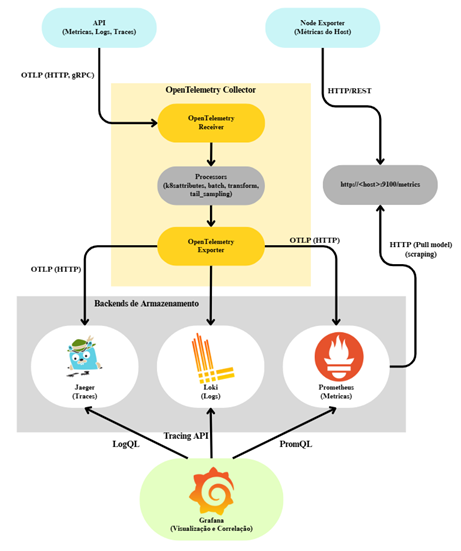
\includegraphics[width=0.8\textwidth]{images/Diagramas/arquitetura_da_solucao.png}
    \caption{Arquitetura da Solução}
    % \label{fig:digital_twin}
\end{figure}

A imagem detalha o fluxo de dados de telemetria desde a sua origem nos micros-serviços até a visualização final no Grafana. A arquitetura é composta pelas se-guintes camadas:

\begin{itemize}
    \item \textbf{APIs e SDKs} \\ As APIs (Application Programming Interfaces) definem os con-tratos para a geração e correlação de dados de telemetria. Os SDKs (Software Development Kits) são implementações específicas de linguagem das APIs, fornecendo as ferramentas necessárias para instrumentar o código das aplica-ções. Estes SDKs permitem aos utilizadores gerar dados de telemetria na sua linguagem de programação escolhida e exportá-los para um backend preferenci-al. Incluem bibliotecas de instrumentação que geram dados relevantes a partir de bibliotecas e frameworks populares (por exemplo, requisições HTTP) e dete-tores de recursos que adicionam atributos contextuais (como nome do pod ou namespace em Kubernetes) aos dados de telemetria.(OpenTelemetry Authors, 2025; \cite{Thakur2022})
    
    \item \textbf{Collector} \\ O OpenTelemetry Collector é um componente independente e agnós-tico de fornecedor, concebido para receber, processar e exportar dados de tele-metria. Atua como um hub centralizado para gerir pipelines de telemetria, rece-bendo dados em vários formatos (como OTLP, Prometheus, Jaeger) e encami-nhando-os para um ou mais backends. A sua capacidade de processar e filtrar dados antes da exportação otimiza o fluxo de dados, reduzindo a sobrecarga nas aplicações e melhorando a eficiência geral. (OpenTelemetry Authors, 2025; \cite{Thakur2022})
    
    \item \textbf{Exportadores (Exporters)} \\ Os exportadores são componentes responsáveis por enviar os dados de telemetria (após serem gerados pelas aplicações ou processa-dos pelo Collector) para ferramentas de backend específicas, como Grafana, Jaeger, Prometheus,, Loki ou outros sistemas proprietários. A utilização de ex-portadores OTLP é considerada uma boa prática, pois são concebidos para emi-tir dados OpenTelemetry sem perda de informação e são amplamente suporta-dos por diversas plataformas de observabilidade. (OpenTelemetry Authors, 2025; \cite{Thakur2022})
    
    \item \textbf{Node Exporter} \\ O Node Exporter é utilizado como agente de monitorização a nível do sistema operativo, responsável por expor métricas relacionadas com CPU, memória, disco e rede. Embora não esteja diretamente integrado no pipe-line do OpenTelemetry Collector, este componente fornece ao Prometheus da-dos cruciais sobre a infraestrutura subjacente, permitindo complementar a ob-servabilidade das aplicações com indicadores do ambiente de execução.
    
    \item \textbf{Camada de Visualização e Análise} \\ O Grafana atua como a interface de usuá-rio unificada para visualizar e analisar os dados. Ele se integra aos backends (Prometheus, Loki e Jaeger), permitindo a criação de dashboards interativos que mostram as métricas, logs e traces de maneira correlacionada.
\end{itemize}


A separação entre instrumentação (APIs e SDKs), processamento/exportação (Collector e Exportadores) e visualização confere maior flexibilidade e desacopla-mento, permitindo que as aplicações permaneçam independentes da infraestrutura de observabilidade subjacente.


\subsection{Fluxo de Telemetria}

O fluxo de dados de telemetria segue um pipeline bem definido:

\begin{enumerate}
    \item A aplicação ASP.NET Core emite dados de observabilidade (logs, métri-cas, traces) através do protocolo OTLP gRPC, e envia-os para o receiver do OpenTelemetry Collector;
    \item As métricas do sistema operativo são recolhidas diretamente pelo Promet-heus através do Node Exporter;
    \item O OTel Receiver aceita entradas de diferentes fontes, incluindo OTLP e scraping Prometheus;
    \item Os dados são então encaminhados para os processadores do Collector, que executam tarefas de transformação (transform), enriquecimento com dife-rentes atributos (attributes), agregação (batch) e amostragem de traces (tail\_sampling);
    \item Após o processamento, os dados são enviados pelo OTel Exporter para os seus respetivos destinos: Logs → Loki, Traces → Jaeger e Métricas → Prometheus;
    \item O Grafana atua como ponto de agregação visual, utilizando as linguagens de consulta específicas de cada backend para gerar dashboards interativos e correlacionados.
\end{enumerate}

\section{Detalhes Técnicos da Implementação}

\subsection{Estratégia de Instrumentação em .NET}

Do ponto de vista técnico, a instrumentação foi aplicada exclusivamente aos servi-ços criados internamente, evitando a recolha de dados de dependências externas. Desta forma, métricas, logs e traces refletem apenas o comportamento dos micro-serviços proprietários, reduzindo o ruído e a sobrecarga de dados. Esta abordagem garante que a telemetria recolhida é relevante para a análise e otimização da plata-forma, focando a monitorização nos elementos críticos sob responsabilidade direta da equipa de desenvolvimento.

A instrumentação de aplicações é um passo crucial para gerar dados de teleme-tria significativos. Em ambientes de microserviços com múltiplas APIs, a instru-mentação individual de cada serviço pode ser repetitiva e propensa a erros, para mitigar esta complexidade, foi adotada uma abordagem prática e reutilizável para a instrumentação de APIs ASP.NET Core, utilizando um pacote comum (DTX.Base.Common). Este pacote encapsula toda a configuração necessária para a emissão de traces distribuídos, métricas e logs estruturados, promovendo uma padronização e um desacoplamento eficaz entre o código da aplicação e a infraes-trutura de observabilidade.
Esta estratégia centraliza a lógica de observabilidade num único ponto, reduzin-do significativamente o código repetido. A configuração da observabilidade pode ser ativada e controlada dinamicamente através de variáveis de ambiente, o que confere grande flexibilidade e portabilidade entre diferentes ambientes (desenvol-vimento, homologação e produção). Para instrumentar novos serviços, a interven-ção é mínima: basta adicionar o pacote DTX.Base.Common, invocar um método de extensão no Program.cs e definir as variáveis de ambiente necessárias.
A lógica de observabilidade foi centralizada num único método de extensão, aplicada na inicialização de cada API .Net:

builder.ConfigureOpenTelemetry();

Este método ativa automaticamente os componentes do OpenTelemetry para instrumentação de tracing distribuído, coleta de métricas e exportação de logs es-truturados. As configurações são controladas dinamicamente por variáveis de am-biente, o que facilita a portabilidade entre diferentes ambientes, sem a necessidade de recompilação ou reconfiguração manual.

\begin{table}[H]
\centering
\caption{Variáveis de ambiente para configuração OTLP Exporter (colocar as em uso)}
\label{tab:otlp_exporter_env_vars}
\begin{tabular}{|p{6cm}|p{8cm}|}
\hline
\textbf{Variável} & \textbf{Descrição} \\
\hline
OTEL\_EXPORTER\_OTLP\_ENDPOINT & URL do collector OTLP \\
\hline
OTEL\_EXPORTER\_OTLP\_PROTOCOL & Protocolo utilizado (grpc ou http/protobuf) \\
\hline
OTEL\_EXPORTER\_OTLP\_HEADERS & Cabeçalhos opcionais no formato chave=valor (ex: Authorization=Bearer abc) \\
\hline
\end{tabular}
\end{table}


\subsection{Vantagens da Abstração da Instrumentação OpenTelemetry}

O encapsulamento da lógica de instrumentação no pacote DTx.Base.Common e a exposição via um método de extensão (ConfigureOpenTelemetry()) proporcionam benefícios significativos para o desenvolvimento e a operação de aplicações distri-buídas:

\begin{itemize}
    \item Padronização da Instrumentação entre Múltiplas APIs: Garante que todas as APIs sigam as mesmas convenções de observabilidade, resultando em dados de telemetria consistentes e facilmente comparáveis. Isso é fundamental para a cor-relação eficaz de dados em sistemas complexos;
    \item Desacoplamento da Infraestrutura de Observabilidade: O código da aplica-ção torna-se independente das ferramentas de backend utilizadas (Grafana, Jae-ger, Tempo, etc.). Se houver uma mudança nas ferramentas de observabilidade, as modificações são minimizadas e confinadas à configuração do collector ou às variáveis de ambiente, não exigindo alterações no código da aplicação;
    \item Facilidade de Configuração via Ambiente: A ativação e o ajuste da observabi-lidade são feitos através de variáveis de ambiente, o que simplifica a implanta-ção e a gestão em diferentes ambientes (desenvolvimento, homologação, produ-ção), promovendo a portabilidade;
    \item Redução Significativa de Código Repetido: Ao centralizar a lógica de obser-vabilidade num único ponto, evita-se a duplicação de código em cada novo ser-viço ou API, tornando o processo de instrumentação mais eficiente e menos propenso a erros.
\end{itemize}

Com esta abordagem, a instrumentação de novos serviços pode ser realizada com mínima intervenção, com a adição do pacote DTX.Base.Common, uma chamada simples ao método de extensão no Program.cs e a definição das variáveis de ambi-ente necessárias. Isso acelera o desenvolvimento e garante que a observabilidade seja uma parte integrante do ciclo de vida da aplicação desde o início.

\subsection{Instrumentação Específica do ASP.NET Core}

A instrumentação foi dividida nos três pilares da observabilidade, utilizando bibli-otecas de instrumentação automática para cada um.

\begin{itemize}
    \item Instrumentação de Tracing Distribuído: A instrumentação de rastrea-mento distribuído utiliza bibliotecas que monitoram requisições web, chamadas HTTP e interações com o banco de dados. Esses dados são ex-portados para o Collector.
.tracing
    .AddAspNetCoreInstrumentation()
    .AddHttpClientInstrumentation()
    .AddEntityFrameworkCoreInstrumentation()
    .AddNpgsql();
    \item Coleta de Métricas: A solução também contempla a recolha de métricas relevantes tanto ao nível da aplicação como do ambiente de execução. As métricas são coletadas pelo SDK e enviadas para o Collector.
.metrics
    .AddAspNetCoreInstrumentation()
    .AddHttpClientInstrumentation()
    .AddRuntimeInstrumentation();
    \item Logs Estruturados: A configuração de logs substitui os providers nati-vos de logging do .NET e ativa o OpenTelemetry como destino principal de logs estruturados.
builder.Logging.AddOpenTelemetry(logging =>
{
    logging.IncludeFormattedMessage = true;
    logging.IncludeScopes = true;
    logging.AddOtlpExporter();
});
\end{itemize}

A utilização de logs estruturados permite realizar pesquisas avançadas por atribu-tos, correlacionar mensagens de log com spans e traces, e visualizar os logs num contexto de execução mais rico (e.g., por serviço, requisição ou erro).

\section{Coleta de dados com o OpenTelemetry Collector}

A fase de coleta é o ponto de entrada para os dados de telemetria no pipeline de observabilidade, é responsável por capturar logs, métricas e traces gerados pelas aplicações instrumentadas, agentes sidecar ou ferramentas de terceiros. Esta coleta é feita principalmente através dos receivers do OpenTelemetry Collector, que atu-am como ouvintes ou scrapers, aceitando dados em vários formatos.
O OpenTelemetry Collector, um componente central do ecossistema, funciona como um hub de processamento centralizado, capaz de lidar com múltiplas fontes e destinos de dados, na implementação em questão, o Collector foi configurado para escutar em duas portas principais para o protocolo OTLP:
4317 para gRPC e 4318 para HTTP. Esta configuração permite que as aplica-ções enviem telemetria usando o protocolo de sua preferência, a fase de coleta é crítica para garantir que os dados cheguem de forma consistente e em tempo real ao pipeline de observabilidade.
No ambiente Kubernetes, a implantação do OpenTelemetry Collector foi reali-zada como um DaemonSet. Esta escolha de implantação garante que o Collector seja executado como um agente em cada nó (node) do cluster, em vez de ser um serviço centralizado. Cada instância do DaemonSet Collector, que age como um agente local, recebe a telemetria dos pods que estão no mesmo nó.
A principal vantagem desta abordagem é a redução de latência e a segurança. Ao coletar a telemetria localmente, os dados não precisam viajar pela rede do clus-ter, reduzindo a latência e o risco de congestionamento, além disso, essa arquitetu-ra de agente local é mais resiliente, pois a falha de um agente afeta apenas a coleta de dados de um único nó, enquanto os outros nós continuam a operar normalmen-te. Essa configuração de DaemonSet, combinada com os receivers do Collector, otimiza o fluxo de telemetria e torna-o mais robusto e eficiente

\subsection{Protocolo OTLP (gRPC/HTTP) e Configuração}

O OpenTelemetry Protocol (OTLP) é o protocolo padrão utilizado na plataforma de observabilidade para o transporte de dados de telemetria, como métricas, logs e tracing distribuído. Desenvolvido como parte do ecossistema OpenTelemetry, o OTLP é um protocolo aberto, extensível e eficiente, que permite a comunicação entre aplicações instrumentadas, agentes de coleta (como o OpenTelemetry Collec-tor) e sistemas de backend como Grafana Loki (logs), Jager (traces) e Prometheus (métricas). O protocolo suporta os formatos gRPC e HTTP/protobuf, garantindo flexibilidade de integração com diversos ambientes e ferramentas. Num cluster Kubernetes, o uso do OTLP padroniza a coleta e exportação de dados de observa-bilidade entre os pods e os componentes da infraestrutura de monitoramento, gera assim portabilidade, interoperabilidade e escalabilidade da solução implementada.

\subsection{OpenTelemetry Operator}

Gerir a observabilidade em ambientes Kubernetes pode tornar-se complexo, espe-cialmente quando é necessário configurar múltiplos Collectors, manter consistên-cia de pipelines e aplicar boas práticas de escalabilidade e segurança. Para simpli-ficar esta gestão, a comunidade desenvolveu o OpenTelemetry Operator, um Custom Kubernetes Operator que automatiza o ciclo de vida dos Collectors e a sua configuração.

\subsubsection{Conceito e Arquitetura}

O OpenTelemetry Operator expande o Kubernetes através de Custom Resource Definitions (CRDs), introduzindo novos tipos de recurso que descrevem configu-rações de observabilidade de forma declarativa.
O recurso mais importante é o OpenTelemetryCollector, no qual o utilizador defi-ne, em YAML, as características desejadas do Collector (receivers, processors, exporters e modo de execução). O Operator traduz automaticamente essa especifi-cação em objetos nativos do Kubernetes, como Deployments, DaemonSets ou ConfigMaps.

Dessa forma:

\begin{enumerate}
    \item O programador ou DevOps aplica um manifesto OpenTelemetryCollector;
    \item O Operator valida e cria os recursos Kubernetes correspondentes;
    \item O Collector é implantado de forma consistente e conforme as boas práticas de-finidas pela comunidade.
\end{enumerate}

\subsubsection{Modos de Deploy suportados}

O CRD OpenTelemetryCollector permite escolher o modo de execução do Collec-tor:

\begin{itemize}
    \item DaemonSet: cada nó do cluster executa uma instância do Collector, recolhendo telemetria localmente;
    \item Deployment: uma instância centralizada atua como gateway, agregando e ex-portando dados;
    \item Sidecar: o Collector é implantado junto de cada Pod, garantindo isolamento máximo e baixo acoplamento;
    \item StatefulSet: utilizado em cenários que exigem persistência ou configuração estável.
\end{itemize}

Essa flexibilidade permite ajustar a arquitetura de observabilidade conforme a natureza da carga de trabalho.

\subsubsection{Vantagens do Operator}

\begin{itemize}
    \item Automação: reduz a necessidade de escrever e manter manifestos Kubernetes complexos para cada Collector;
    \item Consistência: garante que todos os Collectors seguem uma configuração centra-lizada e padronizada;
    \item Integração com GitOps: por ser declarativo, integra-se facilmente em fluxos de CI/CD e ferramentas como ArgoCD ou Flux.
\end{itemize}

Evolução contínua: a comunidade mantém o Operator alinhado com novas versões do OpenTelemetry, reduzindo o risco de configuração obsoleta.

\subsection{Abordagem Adotada: DaemonSet (Agente por nodo)}

\subsubsection{Justificação da Escolha}

Optou-se por executar o OpenTelemetry Collector em DaemonSet, de forma a disponibilizar um agente local em cada nó do cluster. 

\begin{figure}[h]
    \centering
    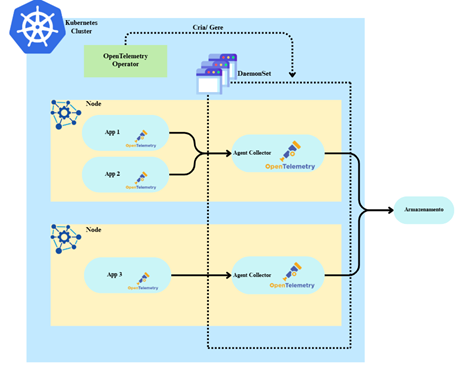
\includegraphics[width=0.8\textwidth]{images/Diagramas/daemonset_collector.png}
    \caption{Implementação de DaemonSet Collector}
    % \label{fig:digital_twin}
\end{figure}

Em cada nó, um Pod do Collector expõe receivers OTLP em gRPC (porta 4317) e HTTP/Protobuf (porta 4318), recebendo métricas, logs e traces das workloads residentes nesse nó. 

Esta opção foi guiada por três objetivos principais:  

\begin{itemize}
    \item Baixa latência na entrega de telemetria, evitando saltos de rede desnecessários antes do primeiro processamento;
    \item Resiliência local, confinando o impacto de falhas ao nó afetado; 
    \item Simplicidade de integração nas aplicações, que passam a publicar telemetria para um endpoint local único.
\end{itemize}

\subsubsection{Beneficios Observados}


A abordagem em DaemonSet resultou em menor variância de entrega dos sinais (coleta e pré-processamento locais), isolamento de falhas por nó, redução da de-pendência de rede intra-cluster e configuração simplificada do lado das aplicações (um único endpoint local, sem descoberta adicional).

\section{Processamento e Transformação dos Dados}

Após a recolha dos dados, estes passam por uma fase crítica de processamento dentro do OpenTelemetry Collector. Esta etapa, orquestrada por vários processa-dores, é essencial para modificar, enriquecer, agrupar ou filtrar os dados, garantin-do a sua compatibilidade e utilidade para os sistemas subsequentes de armazena-mento e análise.

\subsection{Processadores e as suas Aplicações}



\begin{table}[H]
\centering
\caption{Processadores Essenciais do OpenTelemetry Collector}
\label{tab:processadores_otel_collector}
\begin{tabularx}{\textwidth}{|l|X|X|X|}
\hline
\textbf{Processador} & \textbf{Função Primária} & \textbf{Aplicações-Chave} & \textbf{Significado para Observabilidade} \\
\hline
\texttt{transform} & Modifica dados de telemetria usando OTTL. & Adiciona \texttt{service.name}, converte \textit{timestamps}, normaliza severidades de \textit{logs}, aplica regras de amostragem. & Garante consistência dos dados e conformidade com convenções semânticas. \\
\hline
\texttt{batch} & Agrupa dados de telemetria em lotes. & Otimiza a exportação de dados, reduzindo chamadas de rede e sobrecargas. & Melhora o débito e a eficiência do \textit{pipeline}. Crucial para ambientes de alto volume. \\
\hline
\texttt{attributes} & Adiciona, modifica ou elimina atributos (metadados). & Injeta atributos de ambiente estáticos, enriquece com metadados do host. & Enriquece os dados com contexto crucial, melhorando a pesquisa, filtragem e correlação de dados. \\
\hline
\texttt{resource} & Modifica atributos de recurso. & Aplica consistentemente \texttt{service.name} e outros metadados fundamentais. & Assegura a uniformidade de identificadores em todos os dados de telemetria. \\
\hline
\texttt{memory\_limiter} & Previne o consumo excessivo de memória. & Protege o \textit{collector} contra falhas devido ao esgotamento de recursos. & Garante a estabilidade do \textit{pipeline}. \\
\hline
\texttt{tail\_sampling} & Amostra \textit{traces} com base no contexto completo. & Reduz o volume de dados de \textit{trace}, focando-se nos mais críticos (por exemplo, erros ou alta latência). & Otimiza custos de armazenamento e melhora o desempenho de consultas no \textit{backend}. \\
\hline
\end{tabularx}
\end{table}



\begin{itemize}
    \item{Processador transform} \\ Este processador utiliza a OpenTelemetry Transforma-tion Language (OTTL) para realizar modificações extensivas nos dados de te-lemetria. Na implementação atual, é empregado para adicionar o atributo servi-ce.name aos sinais de telemetria, converter timestamps para um formato padro-nizado, normalizar severidades de logs (por exemplo, mapeando vários níveis de log para um conjunto consistente como INFO, WARN, ERROR) e aplicar regras de amostragem dinâmicas a traces. O processador transform é fundamen-tal para garantir a consistência dos dados e a adesão a convenções semânticas predefinidas, o que é primordial para uma análise precisa e uma correlação efi-caz a jusante. Contudo, as suas poderosas capacidades exigem uma configura-ção cuidadosa para evitar "Transformações Inconsistentes" (Unsound Transfor-mations) ou "Conflitos de Identidade" (Identity Conflicts) que possam compro-meter a integridade dos dados;
    
    \item \textbf{Processador batch}  \\ Este processador agrupa eficientemente os dados de tele-metria em lotes antes de serem exportados. O batching reduz significativamente o número de chamadas de rede e a sobrecarga associada, melhorando assim o débito geral e a eficiência da exportação de dados, especialmente em ambientes de alto volume. Processador attributes: Concebido para adicionar, modificar ou eliminar atributos (metadados) em spans, logs ou métricas. Por exemplo, pode ser utilizado para injetar um atributo de ambiente estático (e.g., "produção", "desenvolvimento") em toda a telemetria de entrada ou enriquecer dados com metadados ao nível do host. Este processador é vital para enriquecer os dados de telemetria com informações contextuais cruciais, o que melhora a sua capa-cidade de pesquisa, filtragem e, em última análise, as suas capacidades de corre-lação entre diferentes sinais;
    
    \item \textbf{Processador resource} \\ Tem como alvo específico a modificação de atributos de recurso. Os atributos de recurso descrevem a entidade que produz a telemetria, como o serviço da aplicação, a máquina host ou o contentor. É crucial para ane-xar consistentemente metadados fundamentais como environment, service ver-sion ou region às métricas e para enriquecer logs com informações detalhadas de recurso. Este processador garante que atributos de identificação comuns, no-tavelmente service.name, são aplicados uniformemente em todos os sinais de te-lemetria (logs, traces e métricas). Esta consistência é fundamental para alcançar uma correlação perfeita entre sinais no Grafana;
    
    \item \textbf{Processador memory limiter} \\
    Este processador é implementado para evitar que o OpenTelemetry Collector consuma recursos de memória excessivos. Ao definir limites de memória, impede que o processo do Collector falhe devido ao esgotamento de recursos, garantindo assim a estabilidade e fiabilidade contí-nuas de todo o pipeline de observabilidade;
    
    \item \textbf{Processador tail sampling} \\ Este processador permite decisões de amostragem em traces com base no contexto completo de um trace, ou seja, depois de todos os spans relacionados com um trace terem sido recebidos. Suporta vários crité-rios de filtragem que podem ser encadeados, como amostragem baseada na latência dotrace, taxas probabilísticas, códigos de status HTTP (por exemplo, apenas traces de erro) ou limitação de taxa. A amostragem de cauda é crítica pa-ra gerir o volume de dados de trace, particularmente em sistemas distribuídos de alto tráfego. Ajuda a otimizar os custos de armazenamento e a melhorar o de-sempenho da consulta no backend de tracing sem sacrificar a capacidade de cap-turar e analisar traces críticos ou anómalos.
\end{itemize}


A capacidade do OpenTelemetry Collector de modificar todos os aspetos da tele-metria, incluindo a remoção de informações sensíveis através do processador transform, ou o enriquecimento consistente de dados com atributos específicos, posiciona-o como um ponto de controlo estratégico para a governação de dados. Esta centralização do controlo significa que os requisitos de conformidade podem ser geridos e aplicados ao nível do Collector, reduzindo a necessidade de altera-ções individuais ao nível da aplicação ou de configurações complexas específicas do backend. 
Esta abordagem centraliza significativamente o controlo de dados e minimiza a superfície de ataque para fugas acidentais de dados, além disso, a capacidade de filtrar, agrupar e reduzir a cardinalidade dos dados antes de serem exportados para o backend traduz-se diretamente em poupanças substanciais nos custos de ingestão e armazenamento de dados, especialmente para serviços de observabilidade geri-dos. Ao reduzir o volume e a complexidade dos dados na origem, o Collector me-lhora o desempenho da consulta nos backends e mitiga potenciais problemas de "Crise de Identidade" em métricas, levando a dashboards mais fiáveis. Isto torna o Collector como um componente crítico para gerir tanto a eficiência económica como operacional de toda a pilha de observabilidade.


\section{Persistência e Armazenamento de Dados }

\subsection{Armazenamento de Logs com o Loki}

O Loki foi escolhido como sistema de armazenamento de logs devido à sua arqui-tetura otimizada para consultas baseadas em etiquetas (labels) em vez de full-text search. Esta abordagem torna-o mais eficiente e menos dispendioso em termos de recursos quando comparado com soluções tradicionais, como o Elasticsearch. Os logs estruturados emitidos pelas APIs .NET são enviados ao OpenTelemetry Collector através do protocolo OTLP e, em seguida, exportados para o Loki. A integração nativa com o Grafana permite que os logs sejam visualizados e correla-cionados facilmente com métricas e traces, proporcionando uma análise unificada.

\subsection{Armazenamento de Traces com o Jaeger}

O Jaeger foi adotado como backend de armazenamento e análise de traces distri-buídos, dada a sua capacidade de oferecer visibilidade ponta a ponta sobre o ciclo de vida de uma requisição. Através da identificação do serviço (atributo servi-ce.name), é possível segmentar e filtrar os traces de forma eficaz, identificando gargalos e pontos de falha no percurso entre microserviços. Os dados são exporta-dos pelo OpenTelemetry Collector via protocolo OTLP/gRPC para o endpoint do Jaeger, onde ficam persistidos para consulta e análise detalhada no Grafana.

\subsection{Armazenamento de Métricas com o Prometheus}

O Prometheus foi selecionado como sistema de armazenamento de métricas pela sua robustez no tratamento de séries temporais e pela linguagem de consulta PromQL, que possibilita análises avançadas. As métricas da aplicação .NET são recolhidas pelo OpenTelemetry Collector e exportadas para o Prometheus, centra-lizando a coleta e evitando a exposição direta das aplicações. Complementarmente, métricas de infraestrutura provenientes do Node Exporter são recolhidas direta-mente pelo Prometheus através de scraping HTTP. Esta combinação assegura visi-bilidade tanto a nível da aplicação como da infraestrutura, permitindo uma visão abrangente do desempenho do sistema.
